\section{Character Interactions}
While exploring, the player may focus on an NPC by looking at them from within a certain distance. This will present the player with two options: Talk and Yell. These can be seen in Figure~\ref{fig:UI_npc_talk}.

\subsection{Talk: Conversation}
\label{sec:conversation}
There are two types of conversations the player can have with NPCs in \ourgame{}.

The first type of conversation will be those assigned to only plot-specific characters. While conversing with a plot-specific character, player movement will be disabled and the camera will focus on the NPC. As the character speaks, dialogue is shown in a speech bubble at the top of the screen. These characters will usually have more than one line of dialogue, so the player may manually advance the conversation at any time. During the conversation, the player may occasionally be prompted to choose something to say from a list of dialogue choices. Each choice will be shown as a speech bubble at the bottom of the screen, as shown in Figure~\ref{fig:dialogue}. When a speech bubble is chosen, the conversation will progress according to the player's choice. All of these described conversation elements will be written in the scenario files, and may include triggers for changing player state, affecting the game world, or initiating the yelling contests described in Section~\ref{sec:yelling_contest}.

The second type of conversation triggers when the focused NPC is in a \textbf{non-speaking} state. While in a non-speaking state, the character will speak a single line, shown as text in a speech bubble above their head. This can be seen in Figure~\ref{fig:speech_bubble}. Characters are considered to be in a non-speaking state if they are not involved with any plot events, if they are upset with the player, or they are busy with a particular action. For most characters, this single line will be procedurally generated or selected randomly from a list of pre-written lines. For plot-specific characters, a specific line of dialogue can be written into their scenario. In order to provide variety, multiple lines may exist for a single character and will be cycled through on multiple interactions.

\begin{figure}[H]
  \centering\begin{subfigure}{.45\textwidth}
    \centering
    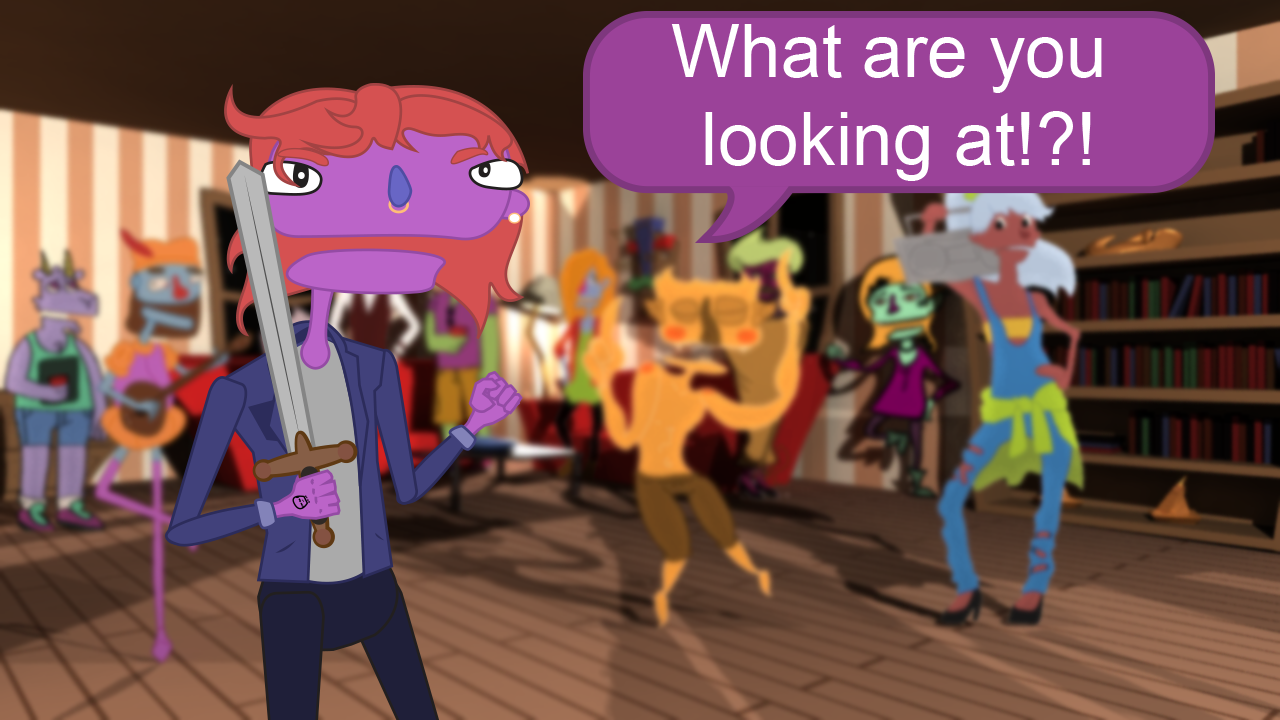
\includegraphics[width=.9\linewidth]{images/UI_npc_nodialogue}
    \caption{Character without dialogue choices}
	\label{fig:speech_bubble}
  \end{subfigure}%
  \begin{subfigure}{.45\textwidth}
    \centering
    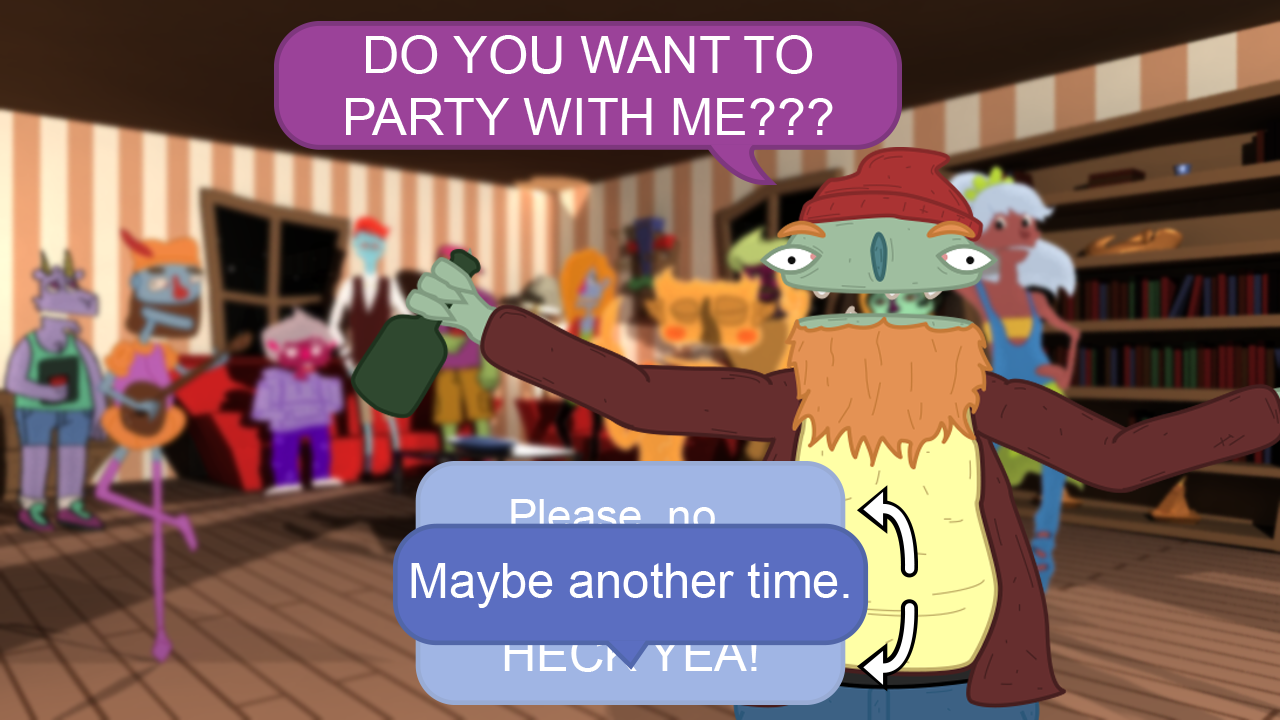
\includegraphics[width=.9\linewidth]{images/UI_npc_conversation}
    \caption{Character with dialogue choices}
	\label{fig:dialogue}
  \end{subfigure}%
  \caption{Characters reacting to talk interactions}
\end{figure}

\subsection{Yell: Yelling Contests}
\label{sec:yelling_contest}

Yelling contests may be initiated in one of two ways: the player may trigger one by intentionally selecting the Yell option while interacting with a character, or they may be triggered by NPCs as part of a scripted sequence. The interaction of a yelling contest can be roughly described as a tug-of-war between the two sides of the conversation, wherein a victor is decided when one side has obliterated the opponent's \textbf{self-confidence}, represented by a shared health bar at the top of the screen.

When an NPC is in \textbf{insult} mode, they will bombard the player with continuous insults, each one damaging the player's self-confidence. This can be seen in Figure~\ref{fig:yelling_contest_a}. In order to gain control, the player is given the opportunity to \textbf{interject} when the NPC pauses at the end of a thought or a sentence. If the player successfully interjects the opposing NPC mid-insult, shown in Figure~\ref{fig:yelling_contest_b}, they will be put into insult mode. While in insult mode, the player will be presented a partial insult with two possible conclusions: One of the presented options will complete the insult, and the other will result in an ineffective insult; an example is given in Figure~\ref{fig:yelling_contest_c}. The player has a limited time to choose the correct conclusion. If the player chooses incorrectly or their time runs out, the opposing NPC will attempt to interject and regain control. If the player chooses correctly, they will tip the scale towards their victory and be presented with another partial insult to complete. The difficulty will increase linearly with the time spent in insult mode by reducing the length of time given to the player to complete insults.

After each battle, the player loses a little bit of their \textbf{voice}. As the player loses more of their voice, they will have less time to complete their insults in the yelling contest. The player can heal themselves by drinking beverages they find around the party. Implementing this limitation adds an extra level of strategy to the yelling contests, and requires the player to be mindful of how they use the Yell option.

\begin{figure}[H]
  \centering\begin{subfigure}{.44\textwidth}
    \centering
    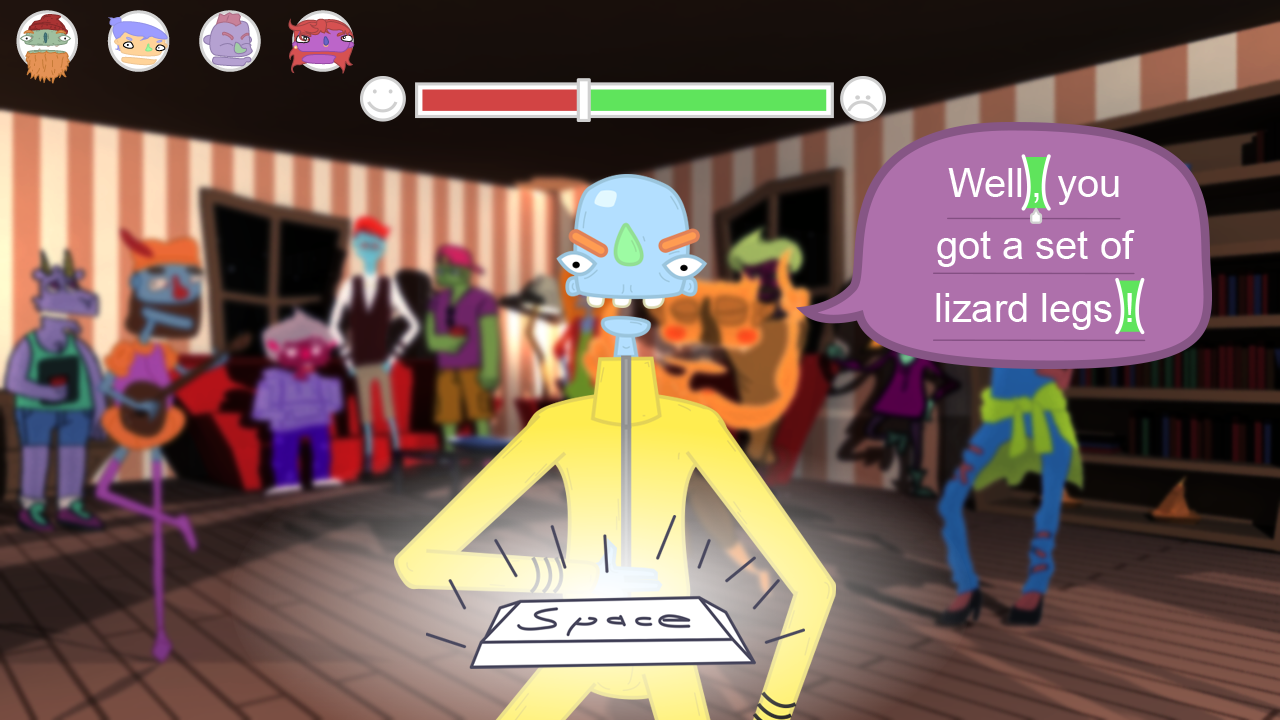
\includegraphics[width=.9\linewidth]{images/UI_yelling_defense}
    \caption{NPC in control - player attempts to interject at highlighted pauses}
    \label{fig:yelling_contest_a}
  \end{subfigure}%
  \begin{subfigure}{.44\textwidth}
    \centering
    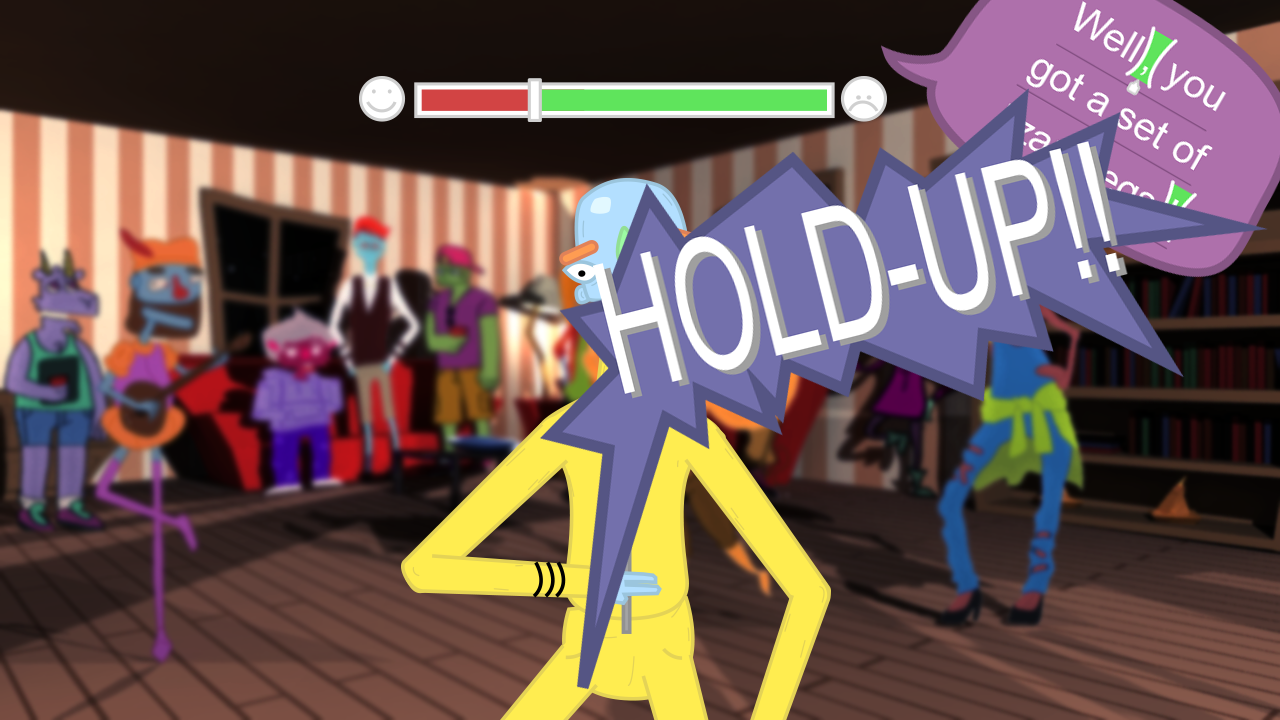
\includegraphics[width=.9\linewidth]{images/UI_yelling_interrupt}
    \caption{Successful interjection by player}
    \label{fig:yelling_contest_b}
  \end{subfigure}
  
  \begin{subfigure}{.44\textwidth}
    \centering
    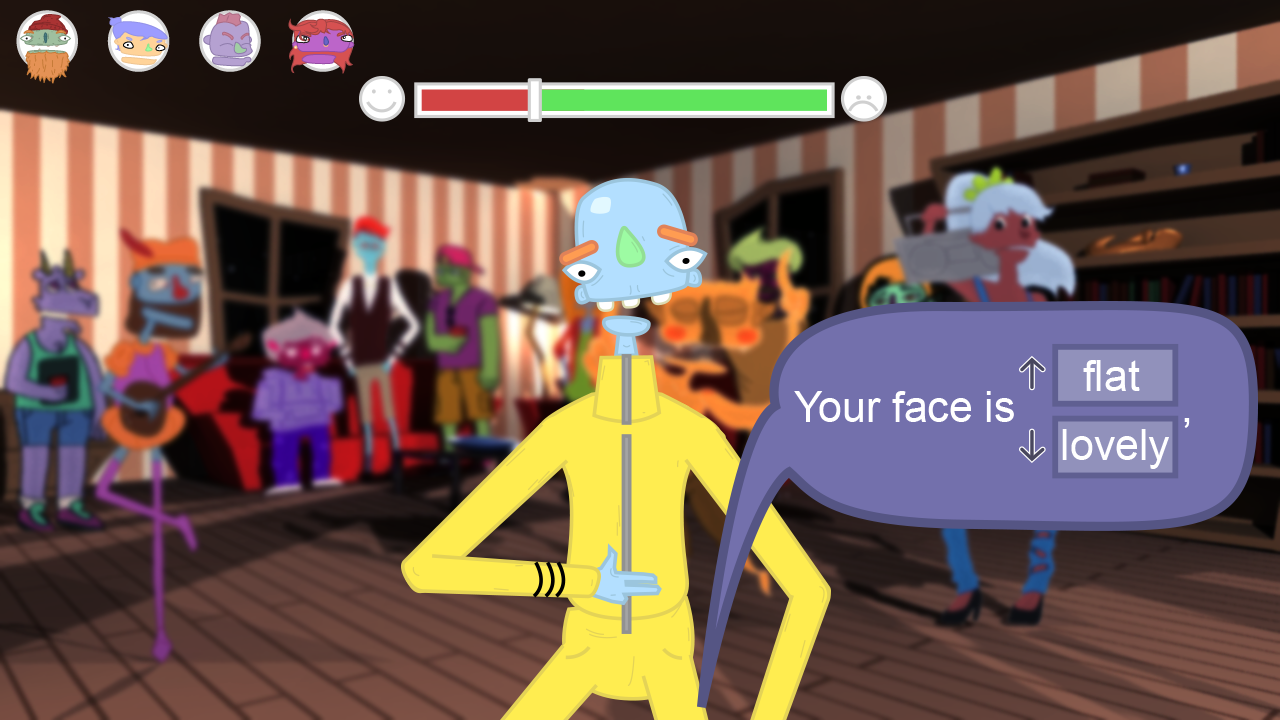
\includegraphics[width=.9\linewidth]{images/UI_yelling_offense}
    \caption{Player in control - player chooses insults instead of compliments while maintaining the rhythm}
    \label{fig:yelling_contest_c}
  \end{subfigure} %
	\begin{subfigure}{.44\textwidth}
	  \centering
	  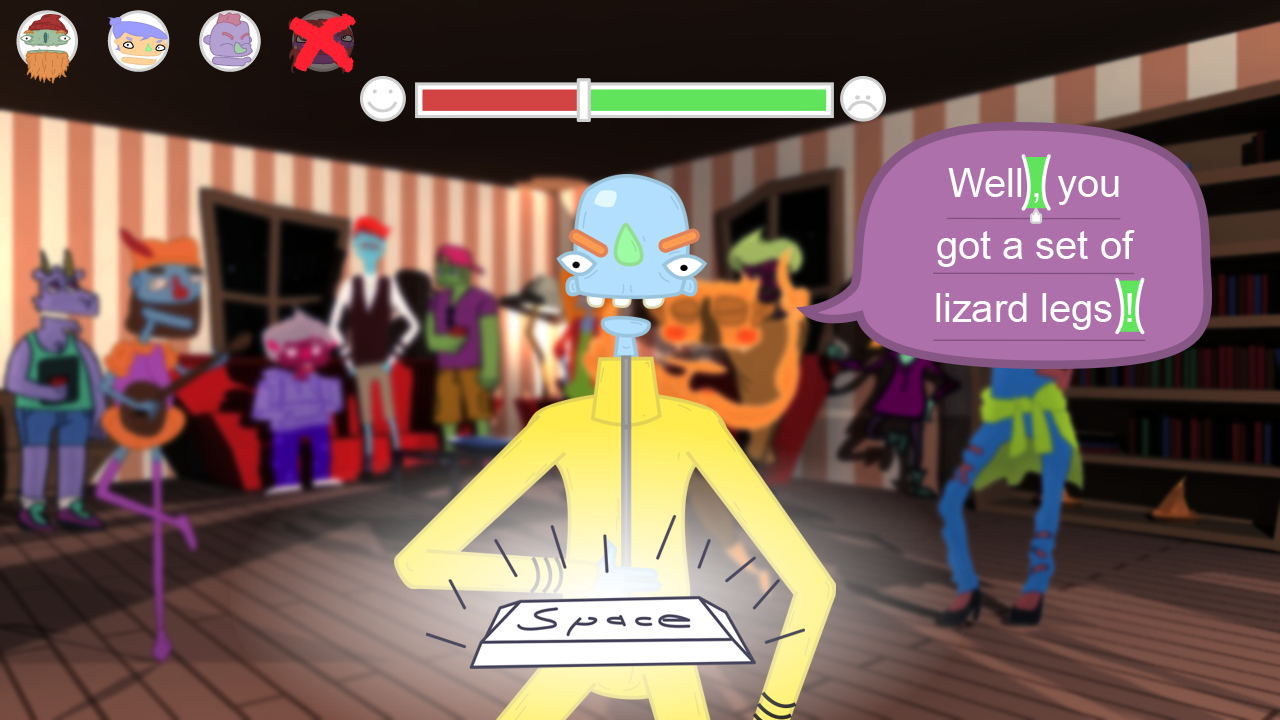
\includegraphics[width=.9\linewidth]{images/UI_yelling_lifelost}
	  \caption{Player with a lost life}
	  \label{fig:yelling_contest_c}
	\end{subfigure}%
  \caption{Yelling Contest mockups}
  \label{fig:yelling_contest}
\end{figure}

\subsubsection{Squads and Followers}
In \ourgame{}, the player can have a squad of NPCs who act as lives during Yelling Contests. These lives are represented by portraits of each NPC in the squad, found in the top-left corner of the screen. The player can recruit NPCs into their squad by completing certain quests. If the player loses the round, the portrait of an NPC will be crossed out to show that they have been used up. If the player loses a round when all member of their squad have been used, they will lose the contest. Upon starting a new yelling contest, any squad members incapacitated in previous matches will be usable again. When the player travels to a different dimension, their squad will become empty.

\subsubsection{D.I.S.S.}
In addition to the player's voice, each character in \ourgame{} will have four primary statistics which affect their performance in yelling contests. Together, these form the D.I.S.S. system. When in yelling contests, the statistics of the active participants will heavily influence the player's ability to win.

\begin{description}
\item[Defense]{decreases damage to the character's self-confidence}
\item[Insight]{makes the correct choice more apparent than the other}
\item[Strength]{increases damage to other character's self-confidence}
\item[Sass]{how long you have to make the correct input (affects how long opponents gaps are)}
\end{description}